\documentclass[12pt, letterpaper]{article}
\renewcommand{\familydefault}{\sfdefault}
\setcounter{secnumdepth}{0}
\usepackage{graphicx}
\title{team retrospection (epic)}
\date{eventually}
\author{melody, mars, and kiri}

\begin{document}
\maketitle
\section{team photo}
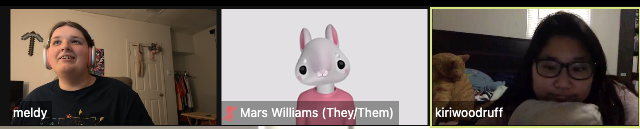
\includegraphics[width=\textwidth]{teamphoto.png}

\section{requirement match}
\begin{table}
\center
\begin{tabular}{|p{5.5in}|p{1in}|}\hline
	\textbf{initial features} & \textbf{implemented?}&\hline
	Users should be able to log children's exercise, including time exercised and type of exercise & Included&\hline
	Should include a page for healthy recipes, with low-cost, simple recipes & Included &\hline
	Includes a daily Recipe of the Day which changes every day &Included&\hline
	Recipes should be filterable by ingredients they include& Included (categories, search)&\hline
	A maze game, similar to the ones the immersive learning project already has on paper&Meh (included the paper)&\hline
	Demonstrations of healthy alternatives to unhealthy choices, and information as to why said choices are unhealthy & Included&\hline
	An `About' page, including information about the immersive learning project from the Henry Gets Moving Delaware County Facebook page, with a picture of the immersive learning team&Included&\hline
	A list of exercises and information about them grouped into sections based on the type&Included&\hline
	An Exercise of the Day which changes every day&Included&\hline
	Users should have an account linked to a username which stores their exercise log data&Included&\hline
	Information about which fruits and vegetables are currently in season to go with the healthy recipes&Not included&\hline
	An administrator section where daily recipes and exercises can be interchanged and the catalogs for each can be updated&Included&\hline
	The app should be accessible to both children and guardians to use&Yep&\hline
	Design elements from the book and the immersive learning project should be included&Yep&\hline
	Include pictures of the characters from the book&Yep&\hline
	Provide a small celebration when 60 minutes of exercise is logged&Yep (trophy)&\hline
	The app should be functional both on desktop and on mobile, as it will primarily be used on iPads&Yep&\hline
	Language written at a pre-school ~ second grade level to be easy for kids to read&Yep&\hline
	Site should be colorful and designed in a way appealing to kids&Yep&\hline

\end{tabular}\caption{requirement match table}
\end{table}
\subsection{If there are missing features in the software, why?}
	The two we missed out on (the maze, fruits/veggies in season) were both marked as low-priority on our requirements list, and the time constraints suggested we would have been better off adding other things and avoiding stepping outside of our knowledge bases. We had a lot of responsibilities on top of adding new features, and we saw other things that would have been useful to our client, that she confirmed were also useful (and were easier to implement).

\section{final meeting and transfer}
\subsection{how did it go?}
	Well enough. Of course, without Nicole having a GitHub account or much experience with software development at all, 
	we didn't have a ton to say, nor anywhere to transfer the repo to besides to you. She asked about deployment, to which 
	we replied it'd probably be done next week, and she said she'd see me (Melody) at the immersive learning showcase on Monday, 
	which I told her I'd go to.

\subsection{\emph{transfer}: how did you do it?}
	Made releases and transferred the repositories to \textbf{hergin} on GitHub. Plan to deploy some time during finals week, probably, 
	which will be the Real transfer, I guess. Also gave Nicole a link to User.md, as she wanted the user manual. Pretty simple stuff, 
	not having a client that works with software.

\section{retrospection}
\subsection{What actions/practices/steps did you take successfully and do them again in your next software project?}
\begin{itemize}
	\item{Task distribution}
	\item{Make good product}
	\item{Put effort into the design and styling and making it look good}
\end{itemize}
\subsection{What actions/practices/steps did you take but you are not happy with the result and wouldn't do them again in your next software project?}
\begin{itemize}
	\item{Time management}
	\item{Worked mostly toward the end of the iteration, e.g.}
\end{itemize}
\subsection{What actions/practices/steps did you miss taking but you would do in your next software project?}
\begin{itemize}
	\item{Issue tracking}
	\item{CI/CD}
	\item{Better frontend testing frameworks that don't break and not spending so much time on it when it does break}
\end{itemize}
\subsection{Suggestions for the future Capstone Teams.}
\begin{itemize}
	\item{Don't overwork yourself}
	\item{Don't go above and beyond, just get it done}
	\item{Distribute work evenly throughout the semester, but don't let that make you feel like you have to do more work}
	\item{Cs get degrees}
\end{itemize}
\subsection{Final thoughts on the project.}
\subsubsection{Each team member will write about how they feel about the status of the project and the two-semester-long process.}
\subsubsection{It can be related to anything about the project.}
\begin{itemize}
	\item{\textbf{Melody}}
	
		For me, personally, it could've gone better. Of course, I learned React, which should be a valuable skill, 
		as all I knew before this class was bare-bones HTML web development from CS 410, but I could have learned 
		React in considerably less painful ways that didn't involve being graded. I liked the \emph{idea} of a 
		two-semester long class that involved working with an external client, but it would have been much better 
		done if it was actually a culmination of everything we'd learned in Ball State thus far instead of just 
		a totally out-of-nowhere project where we're learning entirely new things we've never seen before, while 
		also simultaneously having to implement the things we've been learning since CS 222 that we'll be graded on but that 
		don't necessarily have anything to do with the project. I think we created a great end product, despite the 
		constraints we were placed under, but I don't imagine this'll be the first thing I cite on my résumé, as it 
		wasn't for other alumni I spoke to who took this class that didn't even put it on their résumé before getting 
		hired.
	
	\item{\textbf{Mars}}
	
		I am mostly proud of the work we did for Capstone. I enjoyed working with an external client and being able to create a product from scratch with just myself and two other team members. I think for the time given we created a decent product, though I wouldn't say it's my favourite project I have ever completed. This project was particularly difficult for me due to a wide array of personal health issues that arose during the two semesters we had to work on it, but I still beleive through it all I tried my best. 
	
	\item{\textbf{Kiri}}
	
		I think that this was a good experience to have because it offered me an opportunity to do more different things that my job doesn't offer me. Like I was able to design what the project would look like and made me think of this from a design and ux perspective in addition to a development one. I think that I can put this on my resume as a project that I am proud of because I helped to make it and design it from scratch.
\end{itemize}
\end{document}
